% MIT License

% Copyright (c) 2019 Orange Lee

% Permission is hereby granted, free of charge, to any person obtaining a copy
% of this software and associated documentation files (the "Software"), to deal
% in the Software without restriction, including without limitation the rights
% to use, copy, modify, merge, publish, distribute, sublicense, and/or sell
% copies of the Software, and to permit persons to whom the Software is
% furnished to do so, subject to the following conditions:

% The above copyright notice and this permission notice shall be included in all
% copies or substantial portions of the Software.

% THE SOFTWARE IS PROVIDED "AS IS", WITHOUT WARRANTY OF ANY KIND, EXPRESS OR
% IMPLIED, INCLUDING BUT NOT LIMITED TO THE WARRANTIES OF MERCHANTABILITY,
% FITNESS FOR A PARTICULAR PURPOSE AND NONINFRINGEMENT. IN NO EVENT SHALL THE
% AUTHORS OR COPYRIGHT HOLDERS BE LIABLE FOR ANY CLAIM, DAMAGES OR OTHER
% LIABILITY, WHETHER IN AN ACTION OF CONTRACT, TORT OR OTHERWISE, ARISING FROM,
% OUT OF OR IN CONNECTION WITH THE SOFTWARE OR THE USE OR OTHER DEALINGS IN THE
% SOFTWARE.

\section{从 XML 到 XAML}

\subsection{小试身手:将 TextBlock 换成 Button 试试}

尝试以下代码:
\begin{lstlisting}[language = xml]
    <Grid>
        <Button HorizontalAlignment="Stretch" VerticalAlignment="Stretch" FontSize="72">
            Hello XAML!
        </Button>
    </Grid>
\end{lstlisting}

上面的代码出现了之前没有看到过的 Button。这一步很好解释,我们可以从工具箱里看到 Button,所以知道它不是一件难事。
\begin{figure}[htbp]
    \centering
    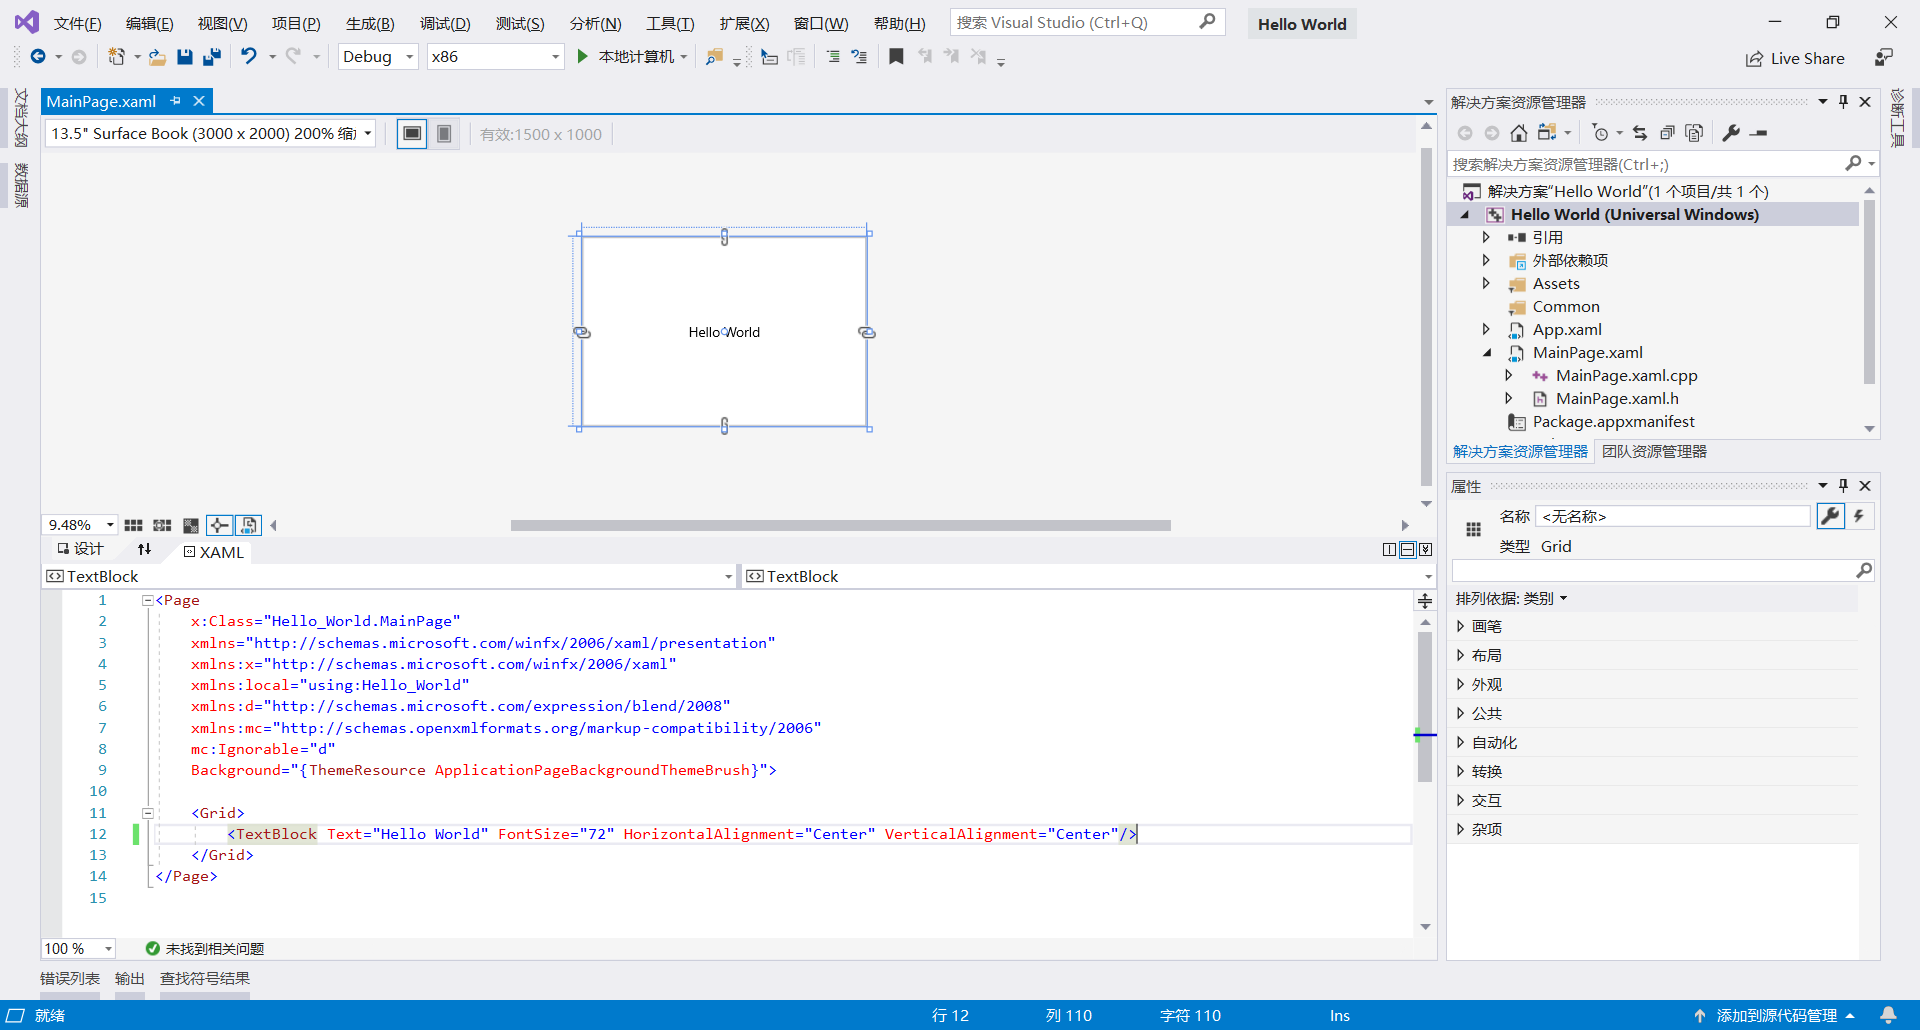
\includegraphics[width = 0.25\paperwidth]{pic/15.png}
    \caption{工具箱有 Button}
\end{figure}

那 \code{"Stretch"} 是从哪里知道的呢?VS 会通过 IntelliSense 的形式提示你。
\begin{figure}[htbp]
    \centering
    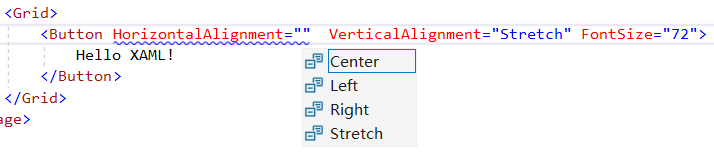
\includegraphics[width = 0.75\paperwidth]{pic/16.png}
    \caption{善用 IntelliSense}
\end{figure}

还有一个问题是,现在这个 Button 有一个文本 \code{Hello XAML!},那这个 Button 还能有子元素吗?尝试以下代码:
\begin{lstlisting}[language = xml]
    <Grid>
        <Button HorizontalAlignment="Stretch" VerticalAlignment="Stretch" FontSize="72">
            <Grid>
                <Button HorizontalAlignment="Stretch" VerticalAlignment="Stretch" FontSize="72">
                    Hello XAML!
                </Button>
            </Grid>
        </Button>
    </Grid>
\end{lstlisting}
\begin{figure}[htbp]
    \centering
    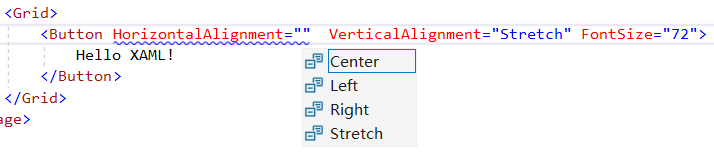
\includegraphics[width = 0.5\paperwidth]{pic/17.png}
    \caption{运行结果}
\end{figure}

那么,还能给外层的 Button 设置文本吗?我们尝试一下:
\begin{figure}[htbp]
    \centering
    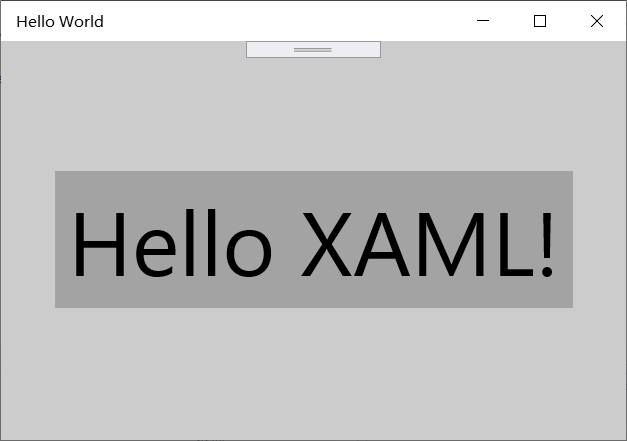
\includegraphics[width = 0.5\paperwidth]{pic/18.png}
    \caption{尝试代码}
\end{figure}
\begin{figure}[htbp]
    \centering
    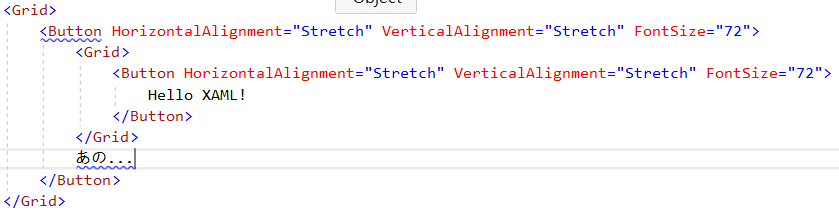
\includegraphics[width = 0.3\paperwidth]{pic/19.png}
    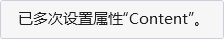
\includegraphics[width = 0.3\paperwidth]{pic/20.png}
    \caption{错误信息}
\end{figure}

为什么会是这样呢?

\subsection{XAML 解惑}

\subsubsection{属性\index{XAML!属性}}

在 XAML 中,元素都具有相应的\emph{属性},例如 Button 拥有一个 \code{HorizontalAlignment} 属性、TextBlock 拥有一个 \code{FontSize} 属性等等。可以通过 XML 中的``属性''来设置这些元素的属性。

\subsubsection{纲要(schema)\index{XML!纲要}\index{XML!schema}}

可以发现,如果给一个元素指定一个不存在的属性,编辑器会提示你发生错误,这是怎么做到的了?事实上,XML 可以使用一种叫做\emph{纲要(schema)}的东西来指定某个元素能拥有哪些子元素等等。关于纲要的内容我们不做深究,只需要知道就是它保证了我们不会在 XAML 编辑器里书写错误的代码。

\subsubsection{默认属性\index{XAML!默认属性}}

对于每个元素,XAML 的纲要都规定了它的\emph{默认属性}。对于默认属性,我们不必以 XML 中``属性''的形式表示,我们可以直接把它放在标签内部,以``文本''或者子元素的形式表示。

根据上面的错误信息,我们很容易就能明白:Button 的默认属性是 Content。如果在标签内部存在一个元素和一个文本,那么相当于 Content 就要设置为一个元素和一个文本,但这是不允许的,根据纲要的规定,Content 只能是一个元素或者是一个文本,因此发生了错误。

我们可以写出以下等价的代码:
\begin{lstlisting}[language = xml]
        <Button HorizontalAlignment="Stretch" VerticalAlignment="Stretch" FontSize="72">
            Hello XAML!
        </Button>
\end{lstlisting}
\begin{lstlisting}[language = xml]
        <Button HorizontalAlignment="Stretch" VerticalAlignment="Stretch" FontSize="72" Content="Hello XAML!"/>
\end{lstlisting}

\subsubsection{通过``子元素''设置 XAML 中元素的属性}

从以上等价的两段代码,我们可以很快发现一个问题:要是 Content 真的像一个 Grid 再嵌套一个 Button 那样复杂,而 Content 又不是默认属性的话,那该如何是好?事实上,还可以通过 XML 的``子元素''来设置 XAML 中元素的属性。见下例:
\begin{lstlisting}[language = xml]
    <Grid>
        <Button>
            <Button.HorizontalAlignment>Stretch</Button.HorizontalAlignment>
            <Button.VerticalAlignment>Stretch</Button.VerticalAlignment>
            <Button.Content>
                <Grid>
                    <TextBlock Text="はい!" FontSize="72"/>
                </Grid>
            </Button.Content>
        </Button>
    </Grid>
\end{lstlisting}

\subsection{顶端的代码}

显然,就是顶端那一长串带有 URL 的代码定义了命名空间。\textbf{我们只需要做到不修改它们就好了。}